% Provenance (never printed): see sources/outline_sources.md (Year 1: gravity and its
% measurement, normal gravity; isostasy, Airy and Pratt; free-air and Bouguer anomalies;
% the geoid). Curves from figdata/bachelor-1/hypsometry.py and gravity_profiles.py;
% exercise and problem values in the Book 3 scratch calculator calc/ch11.py.
\chapter{Isostasia y anomalías de la gravedad}\label{ch:b1:isostasy-gravity}

A comienzos de los años 1840 los topógrafos que medían un arco de meridiano a través del norte de la India se encontraron con una
discrepancia que no podían atribuir a sus instrumentos. Entre dos estaciones distantes unas 370 millas, Kaliana, al pie del
Himalaya, y Kalianpur, mucho más al sur, la diferencia de \omterm{def:b1:spherical-astronomy:geographic}{latitud} obtenida por triangulación superaba en 5.236 segundos de arco la
obtenida a partir de las estrellas. El culpable obvio eran las montañas: su atracción desvía la plomada hacia el norte, y los
astrónomos orientaban sus instrumentos por la plomada. En 1855 John Henry Pratt calculó la atracción del Himalaya y de las mesetas
que lo rodean, y encontró que debía haber producido una discrepancia de 15.885 segundos, más de tres veces lo observado. Las
montañas atraían mucho menos de lo que su masa visible exigía. El mismo año George Airy respondió que la \omterm{def:b1:layered-earth:layers}{corteza} flota sobre una
capa más densa como una balsa de troncos sobre el agua, de modo que las zonas altas tienen una raíz profunda de roca ligera; Pratt
propuso después otra respuesta, una roca aligerada por dilatación bajo las montañas. Ambas se siguen enseñando: las montañas tienen
debajo roca ligera que compensa su masa. Este capítulo convierte esa idea en números, y muestra cómo la gravedad, medida con una
precisión de una millonésima de su valor, revela las masas ocultas bajo el relieve.
% ledger: pratt:himalaya, airy:1855, pratt:1871

\begin{recall}
La ley de gravitación de Newton da el campo $g = GM/r^2$ fuera de una masa esférica $M$; el campo deriva de un potencial
gravitatorio, y una superficie equipotencial es en todas partes perpendicular al campo (física). En un fluido en reposo la presión
crece con la profundidad como $\mathrm dp/\mathrm dz = \rho g$, y un cuerpo flotante desaloja un peso de fluido igual al suyo
(física, primer año universitario). Bajo la \omterm{def:b1:layered-earth:lithosphere}{litosfera} la \omterm{def:b1:layered-earth:lithosphere}{astenosfera} fluye durante tiempos largos; la \omterm{def:b1:layered-earth:layers}{corteza} es más ligera que el
\omterm{def:b1:layered-earth:layers}{manto} que hay debajo (\cref{ch:b1:layered-earth}; libro 2, año 11).
\end{recall}

\section{La gravedad y su medida}

La aceleración de la gravedad en la superficie terrestre es cercana a \qty{9.8}{m.s^{-2}}, y las variaciones que interesan a los
geólogos son un millón de veces menores. Se cuentan en una unidad del antiguo sistema centímetro--gramo, el gal: $\qty{1}{Gal} = \qty{1}{cm.s^{-2}} = \qty{0.01}{m.s^{-2}}$, de modo que
\[
  \qty{1}{\milli\gal} = \qty{e-5}{m.s^{-2}} \approx \num{e-6}\,g .
\]
% ledger: nist:gal
Un instrumento de campo resuelve unas pocas milésimas de miligal; las anomalías estudiadas en este capítulo van desde una fracción de
miligal sobre un yacimiento enterrado hasta unos pocos cientos de miligales sobre una cordillera.

Incluso en una Tierra sin relieve, la gravedad no sería la misma en todas partes. La Tierra gira, de modo que lo que siente una
plomada o un gravímetro es la suma de la atracción gravitatoria y del efecto centrífugo de la rotación; y la Tierra está achatada,
de modo que los polos están más cerca de su centro que el ecuador. Ambos efectos hacen que la gravedad sea más débil en el ecuador
que en los polos. Un geólogo compara cada medida con una referencia suave que las contenga.

\begin{definition}[Gravedad normal]\label{def:b1:isostasy-gravity:normal-gravity}
\emph{Gravedad normal}\index{gravedad normal} $\gamma$ es la gravedad de una Tierra modelo: un elipsoide de revolución con la masa y
la rotación de la Tierra, elegido de modo que su superficie sea una equipotencial de su propia gravedad (gravitación más efecto
centrífugo). Sobre esa superficie, la gravedad normal depende solo de la \omterm{def:b1:spherical-astronomy:geographic}{latitud}.
\end{definition}

El elipsoide mismo, su achatamiento y la forma en que sus parámetros se ajustan a la Tierra real se estudian en el libro de tercer
año universitario. Aquí solo necesitamos su gravedad.

\begin{proposition}[La fórmula de la gravedad normal]\label{prop:b1:isostasy-gravity:normal-formula}
Sobre el elipsoide de referencia adoptado en 1980, la \omterm{def:b1:isostasy-gravity:normal-gravity}{gravedad normal} a la \omterm{def:b1:spherical-astronomy:geographic}{latitud} geográfica $\varphi$ es, en su forma habitual en
serie,
\[
  \gamma(\varphi) = \qty{9.780327}{m.s^{-2}}\,\bigl(1 + 0.0053024\sin^2\varphi
  - 0.0000058\sin^2 2\varphi\bigr).
\]
\end{proposition}
\admitted
% ledger: moritz:grs80

Da \qty{9.780327}{m.s^{-2}} en el ecuador, \qty{9.806200}{m.s^{-2}} a \ang{45} y \qty{9.832186}{m.s^{-2}} en los polos: una
diferencia de \qty{5186}{\milli\gal} entre el ecuador y el polo. La rotación por sí sola explica la mayor parte. Con el día sidéreo de
\qty{23.9345}{h}, la velocidad angular es $\omega = 2\pi/\qty{86164}{s} = \qty{7.292e-5}{rad.s^{-1}}$, y la aceleración centrífuga en
el ecuador, $\omega^2 a$ con $a = \qty{6378.137}{km}$, es \qty{0.0339}{m.s^{-2}}, o \qty{3392}{\milli\gal}; el achatamiento aporta el
resto (\cref{exo:b1:isostasy-gravity:2}).
% ledger: earth:Trot, earth:Req, earth:geq, earth:gpole

La gravedad se mide de dos maneras. Un gravímetro \emph{absoluto} deja caer una masa de prueba en una cámara de vacío y sigue su caída
libre con un interferómetro láser, cronometrada por un reloj atómico: la aceleración sale directamente de la distancia y el tiempo.
Un gravímetro \emph{relativo} es una masa colgada de un resorte, cuyo estiramiento cambia con la gravedad; es ligero y rápido, pero
solo da diferencias entre lugares, y deriva, así que un levantamiento vuelve a una estación base cuya gravedad es conocida. Los mejores
instrumentos absolutos tienen una precisión de unos \qty{1}{\micro\gal}, una parte en mil millones de $g$.
% ledger: ngs:absolute-gravity

\begin{inthefield}[Un levantamiento gravimétrico en el terreno]
\begin{minipage}[t]{0.55\linewidth}\vspace{0pt}
Un levantamiento gravimétrico es una lenta caminata de estación en estación. En cada una el geofísico coloca el gravímetro relativo
sobre su trípode, lo nivela, espera a que el resorte se asiente y toma varias lecturas; un receptor de posicionamiento por satélite
junto a él registra la posición y la altura de la estación. Cada pocas horas el equipo vuelve a la estación base, para medir y
corregir la deriva del resorte. La altura importa tanto como la gravedad: como muestra la sección siguiente, la gravedad disminuye
\qty{0.3086}{\milli\gal} por cada metro de altura, así que una altura equivocada en \qty{1}{cm} estropea la lectura en
\qty{3}{\micro\gal}. % ledger: usgs73:reduction
\end{minipage}\hfill
\begin{minipage}[t]{0.42\linewidth}\vspace{0pt}
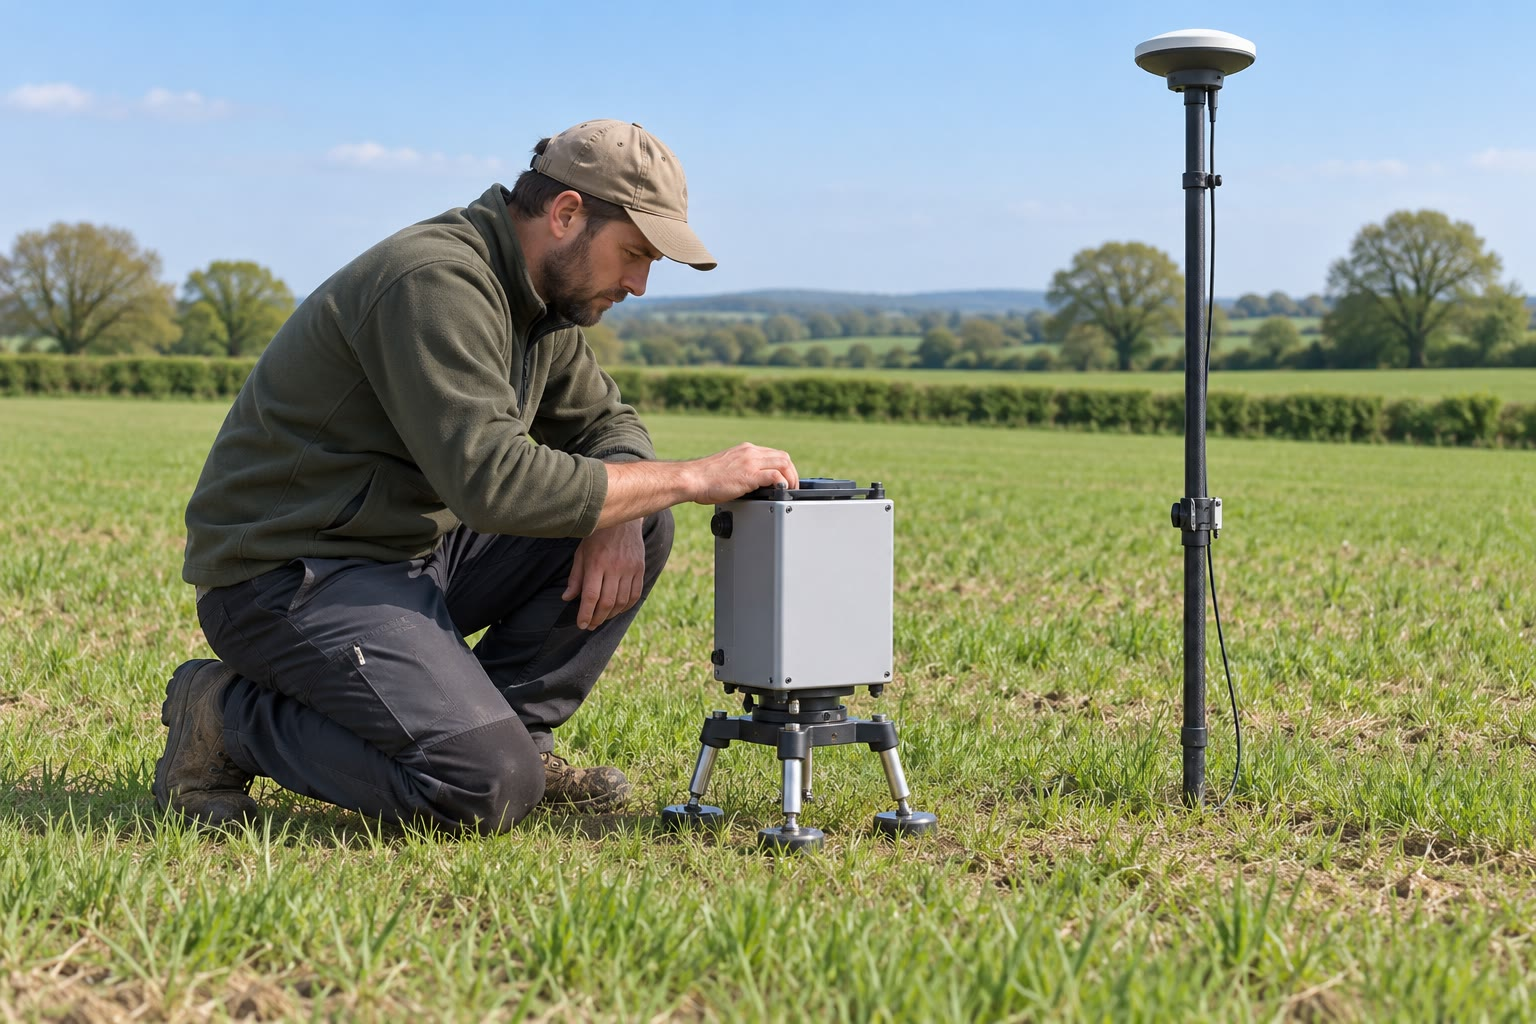
\includegraphics[width=\linewidth]{images/book3/ai/b1-gravity-survey.jpg}

{\scriptsize Un gravímetro de campo sobre su trípode, con una antena de posicionamiento por satélite junto a él (ilustración generada
por IA).}
\end{minipage}
\end{inthefield}

\section{Isostasia}

La compensación que imaginaron Airy y Pratt para el Himalaya es un caso de un estado general de las capas externas de la Tierra.

\begin{definition}[Isostasia; profundidad de compensación]\label{def:b1:isostasy-gravity:isostasy}
Una región está en \emph{isostasia}\index{isostasia}, o equilibrio isostático, cuando existe una profundidad, la \emph{profundidad de
compensación}\index{profundidad de compensación}, a la que la presión es la misma en cada punto de la superficie horizontal, sea cual
sea el relieve por encima. Bajo la profundidad de compensación las rocas se comportan como un fluido en reposo; por encima de ella, las
columnas de \omterm{def:b1:layered-earth:layers}{corteza} y \omterm{def:b1:layered-earth:layers}{manto} flotan sobre él.
\end{definition}

\begin{proposition}[Masas iguales por encima de la profundidad de compensación]\label{prop:b1:isostasy-gravity:equal-mass}
Si la gravedad $g$ es la misma en todas las columnas, una región está en \omterm{def:b1:isostasy-gravity:isostasy}{isostasia} con \omterm{def:b1:isostasy-gravity:isostasy}{profundidad de compensación} $z_c$ si y solo
si cada columna vertical de sección unitaria, desde la superficie hasta $z_c$, contiene la misma masa.
\end{proposition}

\begin{proof}
En cada columna las rocas están en equilibrio hidrostático, de modo que $\mathrm dp/\mathrm dz = \rho(z)\,g$, con la profundidad $z$
contada hacia abajo. La presión en la superficie es la atmosférica, igual en todas partes (y despreciable). Integrando desde la
superficie $z_s$ de la columna hasta $z_c$ se obtiene
\[
  p(z_c) = p_0 + g\int_{z_s}^{z_c}\rho(z)\,\mathrm dz ,
\]
donde la integral es la masa de la columna por unidad de área. Las presiones en $z_c$ son iguales si y solo si lo son estas masas.
\end{proof}

Dos formas sencillas de repartir las masas dan los dos modelos clásicos (figura de abajo).

\begin{proposition}[Isostasia de Airy]\label{prop:b1:isostasy-gravity:airy}
Sea la \omterm{def:b1:layered-earth:layers}{corteza} de densidad uniforme $\rho_c$ y espesor $H$ donde su superficie está al nivel del mar, sobre un \omterm{def:b1:layered-earth:layers}{manto} de densidad
$\rho_m > \rho_c$. En equilibrio isostático:
\begin{enumerate}
  \item donde la superficie se alza una altura $h$ sobre el nivel del mar, la \omterm{def:b1:layered-earth:layers}{corteza} tiene
        una raíz de profundidad $r = h\,\rho_c/(\rho_m - \rho_c)$ bajo la \omterm{def:b1:layered-earth:layers}{corteza} normal,
        y un espesor $H + h + r$;
  \item donde la superficie yace a una profundidad $d$ bajo el nivel del mar, bajo agua de
        densidad $\rho_w$, la \omterm{def:b1:layered-earth:layers}{corteza} tiene una antirraíz: su base se eleva
        $r' = d\,(\rho_c - \rho_w)/(\rho_m - \rho_c)$, y su espesor es
        $H - d - r'$.
\end{enumerate}
Esta es la \emph{isostasia de Airy}\index{isostasia de Airy}: compensación por cambios de espesor a densidad constante.
\end{proposition}

\begin{proof}
Tómese la \omterm{def:b1:isostasy-gravity:isostasy}{profundidad de compensación} justo bajo la raíz más profunda, y compárese cada columna con la normal. (1) La columna alta
tiene \omterm{def:b1:layered-earth:layers}{corteza} en lugar de \omterm{def:b1:layered-earth:layers}{manto} sobre la profundidad $r$, y \omterm{def:b1:layered-earth:layers}{corteza} sobre la altura $h$ donde la columna normal no tiene nada:
masas iguales exigen $\rho_c(h + r) = \rho_m r$, es decir $r(\rho_m - \rho_c) = \rho_c h$. (2) La columna baja tiene agua en lugar de
\omterm{def:b1:layered-earth:layers}{corteza} sobre la profundidad $d$, y \omterm{def:b1:layered-earth:layers}{manto} en lugar de \omterm{def:b1:layered-earth:layers}{corteza} sobre $r'$: masas iguales exigen $\rho_w d + \rho_m r' = \rho_c(d + r')$,
es decir $r'(\rho_m - \rho_c) =
d(\rho_c - \rho_w)$.
\end{proof}

\begin{proposition}[Isostasia de Pratt]\label{prop:b1:isostasy-gravity:pratt}
Sea cada columna terminada en la misma \omterm{def:b1:isostasy-gravity:isostasy}{profundidad de compensación} $D$ bajo el nivel del mar, con densidad uniforme en cada columna,
$\rho_0$ donde la superficie está al nivel del mar. En equilibrio isostático, una columna cuya superficie se alza una altura $h$ tiene
la densidad
\[
  \rho(h) = \rho_0\,\frac{D}{D + h},
\]
y una columna bajo una profundidad $d$ de agua tiene la densidad $\rho = (\rho_0 D - \rho_w d)/(D - d)$. Esta es la \emph{isostasia de
Pratt}\index{isostasia de Pratt}: compensación por cambios de densidad a profundidad constante.
\end{proposition}

\begin{proof}
Masas iguales por encima de $D$: $\rho(h)(D + h) = \rho_0 D$ para la columna alta, y $\rho_w d + \rho(D - d) = \rho_0 D$ para la baja.
\end{proof}

Con $\rho_c = \qty{2700}{kg.m^{-3}}$ y $\rho_m = \qty{3300}{kg.m^{-3}}$, la raíz de Airy es $h\times2700/600 = 4.5\,h$: un relieve
de \qty{2}{km} de altura tiene una raíz de \qty{9}{km}, y una meseta de \qty{4}{km}, una de \qty{18}{km}. En el modelo de Pratt, con
$D = \qty{100}{km}$ y $\rho_0 = \qty{2700}{kg.m^{-3}}$, las mismas dos columnas tienen las densidades 2647 y \qty{2596}{kg.m^{-3}}, dos
y cuatro por ciento más ligeras. Ambos modelos equilibran las mismas masas; difieren en dónde está la roca ligera, y eso lo puede ver
la sismología: Airy predice un \omterm{def:b1:layered-earth:discontinuity}{Moho} que se hunde bajo las montañas, y Pratt uno plano.

\begin{omfigure}
\begin{tikzpicture}[x=0.55cm, y=0.05cm, font=\scriptsize]
% columns computed in calc/ch11.py: Airy roots 9 and 18 km, Pratt densities 2647 and 2596 kg/m3;
% heights above sea level drawn five times larger than depths
\begin{scope}
  \node[font=\small] at (4.5,30) {(a) Airy};
  \fill[omLithGranite!45] (0,0) rectangle (3,-35);
  \fill[omLithGranite!45] (3,10) rectangle (6,-44);
  \fill[omLithGranite!45] (6,20) rectangle (9,-53);
  \fill[omLithPeridotite!45] (0,-35) rectangle (3,-60);
  \fill[omLithPeridotite!45] (3,-44) rectangle (6,-60);
  \fill[omLithPeridotite!45] (6,-53) rectangle (9,-60);
  \draw (0,-60) -- (0,0) -- (3,0) -- (3,10) -- (6,10) -- (6,20) -- (9,20) -- (9,-60);
  \draw (3,0) -- (3,-60) (6,10) -- (6,-60);
  \draw[thick] (0,-35) -- (3,-35) -- (3,-44) -- (6,-44) -- (6,-53) -- (9,-53);
  \draw[densely dashed] (-0.3,-60) -- (9.3,-60);
  \draw[black!50, densely dotted] (-0.3,0) -- (0,0);
  \node[anchor=east] at (-0.3,0) {nivel del mar};
  \node[anchor=east] at (-0.3,-35) {35};
  \node[anchor=east] at (-0.3,-60) {60 km};
  \node at (1.5,-17) {2700}; \node at (4.5,-20) {2700}; \node at (7.5,-24) {2700};
  \node at (1.5,-50) {3300};
  \node[anchor=south] at (1.5,0) {$h = 0$};
  \node[anchor=south] at (4.5,10) {$h = 2$};
  \node[anchor=south] at (7.5,20) {$h = 4$};
  \draw[black!45, densely dotted] (3,-35) -- (9,-35);
  \node at (4.5,-39.5) {raíz 9};
  \node at (7.5,-44) {raíz 18};
\end{scope}
\begin{scope}[xshift=7.9cm]
  \node[font=\small] at (4.5,30) {(b) Pratt};
  \fill[omLithGranite!45] (0,0) rectangle (3,-100);
  \fill[omLithGranite!36] (3,10) rectangle (6,-100);
  \fill[omLithGranite!27] (6,20) rectangle (9,-100);
  \draw (0,-100) -- (0,0) -- (3,0) -- (3,10) -- (6,10) -- (6,20) -- (9,20) -- (9,-100);
  \draw (3,0) -- (3,-100) (6,10) -- (6,-100);
  \draw[densely dashed] (-0.3,-100) -- (9.3,-100);
  \draw[black!50, densely dotted] (-0.3,0) -- (0,0);
  \node[anchor=east] at (-0.3,0) {nivel del mar};
  \node[anchor=east] at (-0.3,-100) {$D = 100$ km};
  \node at (1.5,-50) {2700}; \node at (4.5,-50) {2647}; \node at (7.5,-50) {2596};
  \node[anchor=south] at (1.5,0) {$h = 0$};
  \node[anchor=south] at (4.5,10) {$h = 2$};
  \node[anchor=south] at (7.5,20) {$h = 4$};
\end{scope}
\end{tikzpicture}

\par\smallskip{\small Los dos modelos clásicos de \omterm{def:b1:isostasy-gravity:isostasy}{isostasia}, para tres columnas que se alzan 0, 2 y \qty{4}{km} sobre el nivel del mar
(alturas exageradas cinco veces frente a las profundidades; densidades en \unit{kg.m^{-3}}). (a) Airy: una sola densidad cortical,
con una raíz 4.5 veces la altura. (b) Pratt: una sola \omterm{def:b1:isostasy-gravity:isostasy}{profundidad de compensación}, con columnas más ligeras bajo el terreno más alto.
Cada columna lleva la misma masa por unidad de área sobre la discontinua \omterm{def:b1:isostasy-gravity:isostasy}{profundidad de compensación}.}
\label{fig:b1:isostasy-gravity:models}
\end{omfigure}

La \omterm{def:b1:isostasy-gravity:isostasy}{isostasia} es una afirmación sobre regiones amplias y tiempos largos. La \omterm{def:b1:layered-earth:lithosphere}{astenosfera} cede solo ante cargas que persisten miles de
años, y la \omterm{def:b1:layered-earth:lithosphere}{litosfera} que está encima es lo bastante rígida como para repartir una carga estrecha sobre una región amplia por flexión,
como una tabla soporta un peso: un volcán aislado no tiene por qué estar compensado bajo sí mismo; esta flexión de la \omterm{def:b1:layered-earth:lithosphere}{litosfera} se
estudia en el libro de tercer año universitario. Bajo las grandes cordilleras la \omterm{def:b1:layered-earth:layers}{corteza} es mucho más gruesa que su promedio
continental de unos \qty{30}{km}: el cuadro de Airy, raíces de \omterm{def:b1:layered-earth:layers}{corteza} ligera, es el más cercano para las cordilleras. El de Pratt,
roca más ligera a profundidad constante, explica las dorsales oceánicas, que se elevan sobre un \omterm{def:b1:layered-earth:layers}{manto} superior aligerado por su mayor
temperatura.
% ledger: usgs:crust-thickness

\subsection*{Los dos niveles de la Tierra}

La \omterm{def:b1:isostasy-gravity:isostasy}{isostasia} organiza el relieve de todo el planeta. Su distribución se resume en una sola curva.

\begin{definition}[Curva hipsométrica]\label{def:b1:isostasy-gravity:hypsometry}
La \emph{curva hipsométrica}\index{curva hipsométrica} de un planeta da, para cada fracción $f$ de su superficie, la elevación
$z(f)$ que supera exactamente esa fracción. Es la distribución acumulada de las elevaciones, leída desde arriba.
\end{definition}

Para dibujarla a partir de un modelo de elevaciones en malla, cada celda debe ponderarse por su área. En una malla de un grado de
\omterm{def:b1:spherical-astronomy:geographic}{latitud} y \omterm{def:b1:spherical-astronomy:geographic}{longitud}, la celda comprendida entre las \omterm{def:b1:spherical-astronomy:geographic}{latitudes} $\varphi_1$ y $\varphi_2$ tiene el área
$R^2\,\Delta\lambda\,(\sin\varphi_2 - \sin\varphi_1)$, que se encoge hacia los polos; sumadas todas las celdas, las áreas dan
exactamente $4\pi R^2$. Ordenar las celdas por elevación y acumular sus áreas da la curva de la figura de abajo. Muestra que el
\qty{70.9}{\percent} de la superficie yace bajo el nivel del mar; que la elevación media de las tierras emergidas es de unos
\qty{0.8}{km} y la profundidad media del océano de unos \qty{3.7}{km}; y que la mayor parte de la superficie pertenece a uno de dos
escalones planos, las plataformas continentales cerca del nivel del mar y el fondo abisal entre unos 3.5 y \qty{6}{km} de
profundidad, unidos por una caída abrupta.
% computed in figdata/bachelor-1/hypsometry.py (fraction 0.709, land 793 m, ocean 3692 m); ledger: data:etopo1, wss:ocean-cover

Un planeta con un solo tipo de \omterm{def:b1:layered-earth:layers}{corteza}, con su relieve levantado y desgastado al azar, tendría un solo nivel, con elevaciones
dispersas alrededor de él. La Tierra tiene dos, porque tiene dos tipos de \omterm{def:b1:layered-earth:layers}{corteza} en equilibrio isostático: la \omterm{def:b1:layered-earth:layers}{corteza} continental,
gruesa y ligera, flota alta; la \omterm{def:b1:layered-earth:layers}{corteza} oceánica, delgada y densa, baja (libro 2, año 11). \Cref{exo:b1:isostasy-gravity:8} muestra
que el modelo de Airy con una sola densidad cortical no puede producir ambos niveles con los espesores corticales observados.

\begin{omfigure}
\begin{tikzpicture}
\begin{axis}[omrecord, width=0.84\linewidth, height=6.4cm, xmin=0, xmax=100, ymin=-11, ymax=9,
  xlabel={fracción de la superficie terrestre situada más alta (\unit{\percent})},
  ylabel={elevación (km)}, xtick={0,10,...,100}, ytick={-10,-8,...,8},
  tick label style={font=\scriptsize}, label style={font=\small}, clip=true]
% computed in figdata/bachelor-1/hypsometry.py; ledger: data:etopo1
\addplot[name path=hyps, very thick, black] table[x=area_pc, y expr=\thisrow{elev}/1000] {figdata/out/bachelor-1-hypsometry-curve.dat};
\path[name path=sea] (axis cs:0,0) -- (axis cs:100,0);
\addplot[omSea!60] fill between[of=hyps and sea, soft clip={domain=29.1:100}];
\addplot[omHypsLandC!80] fill between[of=hyps and sea, soft clip={domain=0:29.1}];
\draw[black!60, densely dotted] (axis cs:0,0) -- (axis cs:100,0);
\draw[black!60, densely dashed] (axis cs:29.1,-11) -- (axis cs:29.1,9);
\draw[omSea!60!black, densely dashed] (axis cs:29.1,-3.692) -- (axis cs:100,-3.692);
\draw[omHypsLandF, densely dashed] (axis cs:0,0.793) -- (axis cs:29.1,0.793);
  \node[font=\scriptsize, anchor=south east] at (axis cs:99,0.1) {nivel del mar};
  \node[font=\scriptsize, anchor=south, align=center] at (axis cs:18,1.0) {elevación media\\de las tierras \qty{0.79}{km}};
  \node[font=\scriptsize, anchor=north west, align=left] at (axis cs:31,-3.9) {profundidad media\\del océano \qty{3.69}{km}};
  \node[font=\scriptsize, anchor=north west, align=left] at (axis cs:30.5,6.5) {tierras: \qty{29.1}{\percent}\\de la superficie};
  \node[font=\scriptsize, anchor=north, align=center] at (axis cs:17,-0.5) {plataforma\\continental};
  \node[font=\scriptsize] at (axis cs:62,-5.2) {fondo abisal};
\end{axis}
\end{tikzpicture}

\par\smallskip{\small La \omterm{def:b1:isostasy-gravity:hypsometry}{curva hipsométrica} de la Tierra, a partir del modelo global de relieve ETOPO1 a un grado, con cada celda
ponderada por su área (sobre la Antártida y Groenlandia, la cima del hielo). Los dos tramos casi planos de la curva son las
plataformas continentales cerca del nivel del mar y el fondo oceánico profundo.}
\label{fig:b1:isostasy-gravity:hypsometry}
\end{omfigure}

\section{Anomalías de la gravedad}

\subsection*{Dos correcciones}

Un gravímetro en una colina está más lejos del centro de la Tierra que uno al nivel del mar, y se apoya sobre una capa de roca que el
otro no tiene. Ambos efectos se calculan antes de comparar la medida con la \omterm{def:b1:isostasy-gravity:normal-gravity}{gravedad normal}.

\begin{proposition}[Gradiente de aire libre]\label{prop:b1:isostasy-gravity:free-air}
Fuera de una Tierra esférica de radio $R$, la gravedad disminuye con la altura $h$ a razón de
\[
  \frac{\mathrm dg}{\mathrm dh} = -\frac{2g}{R}\,;
\]
en la superficie, $2g/R \approx \qty{3.08e-6}{s^{-2}}$, unos
\qty{0.308}{\milli\gal} por metro.
\end{proposition}

\begin{proof}
$g(r) = GM/r^2$, así que $\mathrm dg/\mathrm dr = -2GM/r^3 = -2g(r)/r$; en $r = R$, con $g = \qty{9.820}{m.s^{-2}}$ y
$R = \qty{6371}{km}$, $2g/R =
\qty{3.083e-6}{s^{-2}}$.
\end{proof}
% ledger: earth:gmean, earth:Rmean

El achatamiento y la rotación cambian ligeramente el gradiente; el valor que se usa en la práctica es
\qty{0.3086}{\milli\gal.m^{-1}}.
% ledger: usgs73:reduction

\begin{proposition}[Placa de Bouguer]\label{prop:b1:isostasy-gravity:slab}
Una placa horizontal infinita de espesor $h$ y densidad uniforme $\rho$ atrae a un punto exterior con la aceleración vertical
\[
  g_B = 2\pi G\rho h ,
\]
cualquiera que sea la distancia del punto a la placa. Numéricamente $2\pi G =
\qty{0.0419}{\milli\gal}$ por metro de espesor y por cada \qty{1000}{kg.m^{-3}} de densidad.
\end{proposition}

\begin{proof}
Sitúese el punto en el origen y córtese la placa en anillos delgados coaxiales con la vertical que pasa por él. Un anillo a la
distancia $z$ bajo el punto, de radio
$s$, anchura $\mathrm ds$ y espesor $\mathrm dz$, tiene la masa
$\rho\,2\pi s\,\mathrm ds\,\mathrm dz$, toda ella a la distancia $\sqrt{s^2 + z^2}$;
por simetría su atracción es vertical, igual a la atracción de cada
elemento por el coseno $z/\sqrt{s^2+z^2}$ de su ángulo con la vertical:
\[
  \mathrm dg = G\,\frac{\rho\,2\pi s\,\mathrm ds\,\mathrm dz}{s^2 + z^2}\,
  \frac{z}{\sqrt{s^2 + z^2}} .
\]
Para una capa, $\int_0^\infty s\,(s^2 + z^2)^{-3/2}\,\mathrm ds =
\bigl[-(s^2 + z^2)^{-1/2}\bigr]_0^\infty = 1/z$, así que la capa atrae con
$2\pi G\rho\,\mathrm dz$, independientemente de $z$. Sumando las capas en el
espesor $h$ resulta $2\pi G\rho h$. Con $G = \qty{6.674e-11}{m^3.kg^{-1}.s^{-2}}$,
$2\pi G\times\qty{1000}{kg.m^{-3}}\times\qty{1}{m} = \qty{4.19e-7}{m.s^{-2}} =
\qty{0.0419}{\milli\gal}$.
\end{proof}
% ledger: const:G

\begin{definition}[Anomalías de la gravedad]\label{def:b1:isostasy-gravity:anomalies}
Sea $g$ la gravedad medida en una estación de \omterm{def:b1:spherical-astronomy:geographic}{latitud} $\varphi$ y altura $h$ sobre el nivel del mar.
\begin{itemize}
  \item Una \emph{anomalía de la gravedad}\index{anomalía de la gravedad} es la diferencia entre la gravedad medida, corregida a un
        nivel común, y la \omterm{def:b1:isostasy-gravity:normal-gravity}{gravedad normal} a la misma \omterm{def:b1:spherical-astronomy:geographic}{latitud}.
  \item La \emph{corrección de aire libre}\index{corrección de aire libre} es
        $+\qty{0.3086}{\milli\gal.m^{-1}}\times h$: restituye la disminución de la gravedad con la altura. La \emph{anomalía de
        aire libre}\index{anomalía de aire libre} es
        $\Delta g_{\mathrm{FA}} = g + 0.3086\,h - \gamma(\varphi)$.
  \item La \emph{corrección de Bouguer}\index{corrección de Bouguer} es $-2\pi G\rho h$: elimina la atracción de la roca entre la
        estación y el nivel del mar, tratada como una placa de densidad $\rho$, convencionalmente \qty{2670}{kg.m^{-3}}, lo que da
        \qty{0.112}{\milli\gal} por metro. La \emph{anomalía de Bouguer}\index{anomalía de Bouguer} es
        $\Delta g_{\mathrm B} = \Delta g_{\mathrm{FA}} - 2\pi G\rho h$.
\end{itemize}
\end{definition}
% ledger: usgs73:reduction, swisstopo:bouguer-map

La placa es un modelo grosero del terreno alrededor de una estación en un país accidentado: los valles bajo la estación se cuentan
como roca que no está, y las colinas por encima de ella tiran hacia arriba y no se cuentan en absoluto. Una tercera reducción, la
corrección del terreno, calculada a partir de un \omterm{def:b1:geological-maps:dem}{modelo digital de elevaciones}, elimina ambos errores. En el mar la \omterm{def:b1:isostasy-gravity:anomalies}{corrección de
aire libre} se anula, y la reducción de Bouguer sustituye el agua por roca.

\begin{method}[Reducción de una lectura de gravedad]\label{met:b1:isostasy-gravity:reduction}
\begin{enumerate}
  \item Calcúlese la \omterm{def:b1:isostasy-gravity:normal-gravity}{gravedad normal} $\gamma(\varphi)$ a la \omterm{def:b1:spherical-astronomy:geographic}{latitud} de la estación.
  \item Súmese a la gravedad medida la \omterm{def:b1:isostasy-gravity:anomalies}{corrección de aire libre} $0.3086\,h$ (en \unit{\milli\gal}, con $h$
        en metros) y réstese $\gamma$: esta es la \omterm{def:b1:isostasy-gravity:anomalies}{anomalía de aire libre}.
  \item Réstese la \omterm{def:b1:isostasy-gravity:anomalies}{corrección de Bouguer} $0.0419\times(\rho/1000)\times h$, es decir
        $0.112\,h$ para la densidad estándar: esta es la \omterm{def:b1:isostasy-gravity:anomalies}{anomalía de Bouguer}.
  \item Trabájese en miligales en todo momento, y consérvense la gravedad medida y la normal con siete cifras significativas: la
        anomalía es una pequeña diferencia de dos números grandes.
\end{enumerate}
\end{method}

\begin{example}[Una estación en las colinas]\label{ex:b1:isostasy-gravity:reduction}
En una estación a \omterm{def:b1:spherical-astronomy:geographic}{latitud} \ang{45} y \qty{1200}{m} sobre el nivel del mar, el gravímetro da \qty{9.802597}{m.s^{-2}}. La \omterm{def:b1:isostasy-gravity:normal-gravity}{gravedad
normal} allí es \qty{9.806200}{m.s^{-2}}; el valor medido es menor en \qty{360.3}{\milli\gal}.
La \omterm{def:b1:isostasy-gravity:anomalies}{corrección de aire libre} es $0.3086\times1200 = \qty{370.3}{\milli\gal}$, así que
$\Delta g_{\mathrm{FA}} = -360.3 + 370.3 = \qty{+10.0}{\milli\gal}$. La \omterm{def:b1:isostasy-gravity:anomalies}{corrección de Bouguer}
es $0.112\times1200 = \qty{134.4}{\milli\gal}$, así que $\Delta g_{\mathrm B}
= \qty{-124.4}{\milli\gal}$: hay menos masa bajo esta estación que bajo una estación al nivel del mar, una vez eliminada la roca
sobre el nivel del mar.
\end{example}

\subsection*{Lo que las anomalías dicen sobre la compensación}

\begin{proposition}[Anomalías sobre un relieve amplio]\label{prop:b1:isostasy-gravity:broad}
Considérese una meseta de altura $h$ y densidad $\rho_c$, mucho más ancha que su \omterm{def:b1:isostasy-gravity:isostasy}{profundidad de compensación}, y una estación cerca de
su centro. Tómese la densidad de Bouguer igual a $\rho_c$.
\begin{enumerate}
  \item Si la meseta no está compensada, $\Delta g_{\mathrm{FA}} \approx
        2\pi G\rho_c h$ y $\Delta g_{\mathrm B} \approx 0$.
  \item Si está en equilibrio isostático, sea cual sea la distribución de las masas compensadoras,
        $\Delta g_{\mathrm{FA}} \approx 0$ y $\Delta g_{\mathrm B} \approx -2\pi G\rho_c h$.
\end{enumerate}
\end{proposition}

\begin{proof}
La \omterm{def:b1:isostasy-gravity:normal-gravity}{gravedad normal} a la altura de la estación es $\gamma - 0.3086\,h$, así que la \omterm{def:b1:isostasy-gravity:anomalies}{anomalía de aire libre} es la atracción de las
masas que difieren de las de una columna normal. Cerca del centro de una meseta amplia, cada capa de estas masas anómalas actúa
como una placa infinita, y por \cref{prop:b1:isostasy-gravity:slab} una placa de contraste de densidad $\Delta\rho$ y espesor $t$
atrae con $2\pi G\Delta\rho
t$ dondequiera que esté. El total es $2\pi G$ por la masa anómala por unidad de área. (1) Sin compensación esa masa es $\rho_c h$.
(2) En \omterm{def:b1:isostasy-gravity:isostasy}{isostasia} es cero por \cref{prop:b1:isostasy-gravity:equal-mass}. En ambos casos la \omterm{def:b1:isostasy-gravity:anomalies}{corrección de Bouguer} resta $2\pi G\rho_c h$.
\end{proof}

En la compensación de Airy, la \omterm{def:b1:isostasy-gravity:anomalies}{anomalía de Bouguer} del segundo caso es también $-2\pi G(\rho_m - \rho_c)r$, la atracción de la masa
que falta en la raíz, ya que $(\rho_m - \rho_c)r = \rho_c h$. Las \omterm{def:b1:isostasy-gravity:anomalies}{anomalías de aire libre} cercanas a cero sobre regiones amplias son
así la señal de la \omterm{def:b1:isostasy-gravity:isostasy}{isostasia}, y las \omterm{def:b1:isostasy-gravity:anomalies}{anomalías de Bouguer} que siguen el relieve como imagen especular miden las masas compensadoras:
las \omterm{def:b1:isostasy-gravity:anomalies}{anomalías de Bouguer} son regionalmente negativas a lo largo de los Alpes, y sobre las dorsales oceánicas, por elevadas que estén,
la \omterm{def:b1:isostasy-gravity:anomalies}{anomalía de aire libre} es pequeña. Sobre los océanos la \omterm{def:b1:isostasy-gravity:anomalies}{anomalía de Bouguer} es positiva: sustituir el agua por roca añade masa
sobre una columna a la que no le falta ninguna.
% ledger: swisstopo:bouguer-map

Cerca de los bordes del relieve la aproximación de la placa falla, porque el relieve está cerca de la estación y la raíz muy por
debajo de ella. La figura de abajo da la atracción exacta de una cordillera modelo de \qty{200}{km} de anchura y \qty{2}{km} de
altura. Sin compensación, la \omterm{def:b1:isostasy-gravity:anomalies}{anomalía de aire libre} es \qty{+225}{\milli\gal} en el centro, cerca del valor de la placa,
\qty{226}{\milli\gal}; con una raíz de Airy de \qty{9}{km}, la \omterm{def:b1:isostasy-gravity:anomalies}{anomalía de aire libre} central cae a \qty{+55}{\milli\gal}, no a cero,
porque una cordillera de solo \qty{200}{km} de anchura no parece infinita desde \qty{40}{km} por encima de su raíz, y la \omterm{def:b1:isostasy-gravity:anomalies}{anomalía de
aire libre} se vuelve bruscamente negativa justo más allá de cada borde, donde la estación ve la raíz pero no la montaña.
% computed in figdata/bachelor-1/gravity_profiles.py (centre values 225.0, -1.4, 55.2, -171.2 mGal)

\begin{omfigure}
\begin{tikzpicture}
\begin{axis}[omrecord, name=anom, width=0.86\linewidth, height=6.2cm, xmin=-300, xmax=300, ymin=-310, ymax=250,
  ylabel={anomalía (\unit{\milli\gal})}, xticklabels={}, ytick={-200,-100,0,100,200},
  tick label style={font=\scriptsize}, label style={font=\small},
  legend style={font=\scriptsize, at={(0.01,0.01)}, anchor=south west, draw=none, fill=white, fill opacity=0.85, text opacity=1},
  legend cell align=left, legend columns=2]
% computed in figdata/bachelor-1/gravity_profiles.py
\addplot[very thick, red!75!black] table[x=x, y=fa_unc] {figdata/out/bachelor-1-gravity_profiles-profiles.dat};
\addlegendentry{aire libre, sin compensar}
\addplot[thick, red!75!black, densely dashed] table[x=x, y=bg_unc] {figdata/out/bachelor-1-gravity_profiles-profiles.dat};
\addlegendentry{Bouguer, sin compensar}
\addplot[very thick, blue!70!black] table[x=x, y=fa_airy] {figdata/out/bachelor-1-gravity_profiles-profiles.dat};
\addlegendentry{aire libre, raíz de Airy}
\addplot[thick, blue!70!black, densely dashed] table[x=x, y=bg_airy] {figdata/out/bachelor-1-gravity_profiles-profiles.dat};
\addlegendentry{Bouguer, raíz de Airy}
\draw[black!50, densely dotted] (axis cs:-300,0) -- (axis cs:300,0);
\end{axis}
\begin{axis}[at={(anom.south west)}, anchor=north west, yshift=-0.25cm, width=0.86\linewidth, height=3.6cm,
  xmin=-300, xmax=300, ymin=-50, ymax=5, axis background/.style={fill=white},
  xlabel={distancia al centro de la cordillera (km)}, ylabel={profundidad (km)},
  ytick={0,-35,-44}, yticklabels={0,35,44}, tick label style={font=\scriptsize}, label style={font=\small}]
\fill[omLithPeridotite!45] (axis cs:-300,-50) rectangle (axis cs:300,-35);
\fill[omLithGranite!45] (axis cs:-300,-35) rectangle (axis cs:300,0);
\fill[omLithGranite!45] (axis cs:-100,0) rectangle (axis cs:100,2);
\fill[omLithGranite!45, pattern color=blue!60!black, postaction={pattern=north east lines, pattern color=blue!50!black}] (axis cs:-100,-35) rectangle (axis cs:100,-44);
\draw (axis cs:-300,0) -- (axis cs:-100,0) -- (axis cs:-100,2) -- (axis cs:100,2) -- (axis cs:100,0) -- (axis cs:300,0);
\draw[thick] (axis cs:-300,-35) -- (axis cs:300,-35);
\draw[thick, blue!60!black] (axis cs:-100,-35) -- (axis cs:-100,-44) -- (axis cs:100,-44) -- (axis cs:100,-35);
\node[font=\scriptsize] at (axis cs:-200,-17) {corteza 2700};
\node[font=\scriptsize] at (axis cs:-200,-43) {manto 3300};
\node[font=\scriptsize, fill=white, inner sep=1pt, anchor=west] at (axis cs:105,-40) {raíz de Airy (segundo modelo)};
\node[font=\scriptsize, anchor=south] at (axis cs:0,2) {cordillera, \qty{2}{km} de altura};
\end{axis}
\end{tikzpicture}

\par\smallskip{\small Arriba: \omterm{def:b1:isostasy-gravity:anomalies}{anomalías de aire libre} y de Bouguer a través de una cordillera modelo de \qty{200}{km} de anchura y
\qty{2}{km} de altura, calculadas con exactitud para cuerpos bidimensionales, con estaciones en la superficie del terreno (sin
corrección de terreno). Abajo: el modelo (escala vertical exagerada menos de dos veces); la raíz solo existe en el caso compensado.
Sin compensar, la \omterm{def:b1:isostasy-gravity:anomalies}{anomalía de aire libre} sigue el relieve y la \omterm{def:b1:isostasy-gravity:anomalies}{anomalía de Bouguer} es casi nula; compensada, la \omterm{def:b1:isostasy-gravity:anomalies}{anomalía de aire
libre} es pequeña en el centro con efectos de borde bruscos, y la \omterm{def:b1:isostasy-gravity:anomalies}{anomalía de Bouguer} es un valle amplio.}
\label{fig:b1:isostasy-gravity:profiles}
\end{omfigure}

\begin{method}[Prueba de isostasia de una región]\label{met:b1:isostasy-gravity:test}
\begin{enumerate}
  \item Promédiese la \omterm{def:b1:isostasy-gravity:anomalies}{anomalía de aire libre} sobre un área varias veces más ancha que el espesor de la \omterm{def:b1:layered-earth:layers}{corteza}, lejos de los bordes
        del relieve.
  \item Si está cerca de cero, la región está compensada; si se acerca a $2\pi G\rho_c$ por la altura media, no lo está.
  \item El cociente $-\Delta g_{\mathrm B}/(2\pi G\rho_c h)$ da la fracción del relieve que está compensada.
  \item La evidencia sísmica u otra sobre la profundidad del \omterm{def:b1:layered-earth:discontinuity}{Moho} distingue la compensación de Airy de la de Pratt: la gravedad de
        gran escala por sí sola no puede, ya que ambas ponen el mismo déficit de masa bajo el relieve.
\end{enumerate}
\end{method}

\begin{history}[La gravedad en el mar]
\begin{minipage}[t]{0.58\linewidth}\vspace{0pt}
Un péndulo mide la gravedad a través de su período, pero en un barco las olas lo sacuden mucho más que cualquier anomalía. En los
años 1920 el geodesta neerlandés Felix Vening Meinesz encontró la manera de rodearlo: dos péndulos que oscilan en fase opuesta en un
mismo marco sienten las mismas aceleraciones horizontales del barco, y su diferencia las cancela. Desde 1923 llevó su aparato en
submarinos de la marina neerlandesa, donde, sumergidos, se libraban de lo peor de las olas; primero en un viaje a las Indias
Orientales y después en levantamientos de sus mares. A lo largo de las fosas oceánicas del archipiélago encontró largos cinturones
de anomalías isostáticas fuertemente negativas, y luego las encontró en otras fosas: solo podía explicarlas por una \omterm{def:b1:layered-earth:layers}{corteza} retenida
allí por fuerzas externas, fuera del equilibrio isostático.
% ledger: egs:vening-meinesz
\end{minipage}\hfill
\begin{minipage}[t]{0.38\linewidth}\vspace{0pt}
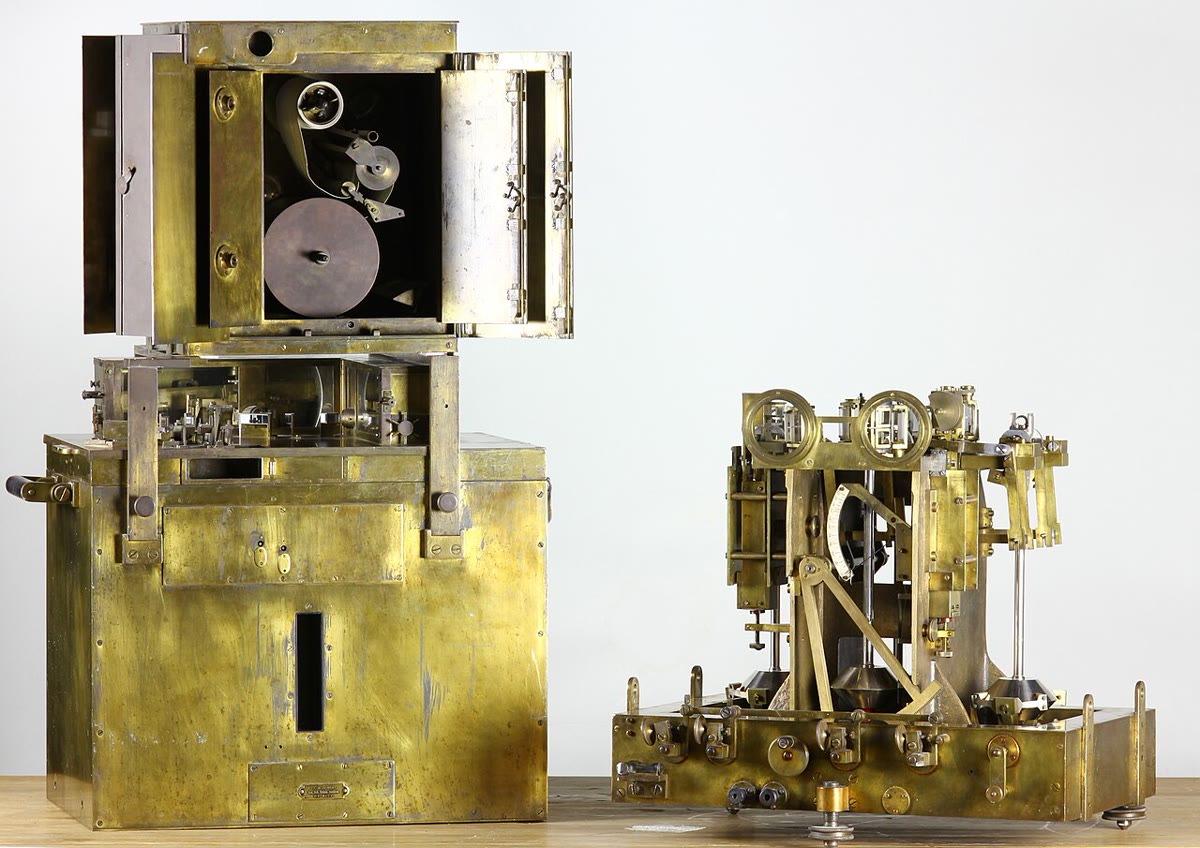
\includegraphics[width=\linewidth]{images/book3/b1-vening-meinesz.jpg}

{\scriptsize Un aparato de péndulo de Vening Meinesz (a la derecha) y su caja con
la unidad de registro (Broodt, CC BY-SA 4.0).}
\end{minipage}
\end{history}

\section{El geoide}

La superficie del mar en reposo es una superficie de potencial gravitatorio constante: si no lo fuera, el agua fluiría a lo largo de
ella. Es la referencia natural para las alturas, y la superficie a la que eran perpendiculares las antiguas plomadas.

\begin{definition}[Geoide; altura del geoide]\label{def:b1:isostasy-gravity:geoid}
El \emph{geoide}\index{geoide} es la superficie equipotencial de la gravedad de la Tierra (gravitación más el efecto centrífugo de la
rotación) que coincide con la superficie media del mar en los océanos abiertos, en reposo, y se prolonga bajo los continentes. La
\emph{altura del geoide}\index{altura del geoide} $N$ en un punto es la altura del geoide sobre el elipsoide de referencia, contada
negativa donde el geoide yace por debajo de él.
\end{definition}

Las alturas sobre el nivel del mar en los mapas son alturas sobre el \omterm{def:b1:isostasy-gravity:geoid}{geoide}; las alturas que dan los sistemas de posicionamiento por
satélite son alturas sobre el elipsoide; ambas difieren en $N$. El \omterm{def:b1:isostasy-gravity:geoid}{geoide} se aparta del elipsoide en \qty{+85}{m} cerca de Islandia y
\qty{-106}{m} frente al sur de la India, menos de \qty{200}{m} en total, mientras que el relieve de la superficie sólida abarca unos
\qty{20}{km}: el \omterm{def:b1:isostasy-gravity:geoid}{geoide} es una superficie mucho más suave que el terreno.
% ledger: nasa:geoid-range, earth:topo

\begin{proposition}[Altura del geoide y anomalía de potencial]\label{prop:b1:isostasy-gravity:bruns}
Sea $\Phi$ el potencial gravitatorio de la Tierra y $\Phi_n$ el potencial normal, el de la Tierra modelo cuya superficie, el elipsoide
de referencia, tiene el mismo potencial $\Phi_0$ que el \omterm{def:b1:isostasy-gravity:geoid}{geoide}, ambos contados con el signo de la física (el potencial crece hacia
arriba y $g = -\nabla\Phi$). Sea $T = \Phi - \Phi_n$ la anomalía de potencial en el \omterm{def:b1:isostasy-gravity:geoid}{geoide}. En primer orden,
\[
  N = -\frac{T}{\gamma} .
\]
Los geodesistas, que cuentan el potencial con el signo opuesto, escriben el mismo resultado como $N = T/\gamma$, la fórmula de Bruns.
\end{proposition}

\begin{proof}
Sea $Q$ un punto del elipsoide y $P$ el punto del \omterm{def:b1:isostasy-gravity:geoid}{geoide} sobre la normal que pasa por $Q$, a la altura $N$. El potencial normal
crece hacia arriba a razón de $\gamma$, así que $\Phi_n(P) \approx \Phi_n(Q) + \gamma N = \Phi_0 +
\gamma N$. Como $P$ está en el \omterm{def:b1:isostasy-gravity:geoid}{geoide}, $\Phi(P) = \Phi_0$, es decir
$\Phi_n(P) + T = \Phi_0$. Por tanto $\Phi_0 + \gamma N + T = \Phi_0$ y $N =
-T/\gamma$.
\end{proof}

Un exceso de masa bajo un punto hace el potencial allí más negativo, así que $T < 0$ y $N > 0$: el \omterm{def:b1:isostasy-gravity:geoid}{geoide} se abomba sobre el exceso
de masa y se hunde sobre un déficit. Los \qty{85}{m} de la elevación cerca de Islandia corresponden a una anomalía de potencial de
$-\qty{85}{m}\times\qty{9.8}{m.s^{-2}} \approx \qty{-830}{J.kg^{-1}}$. Como el potencial decae como $1/r$ mientras que la atracción
decae como $1/r^2$, el \omterm{def:b1:isostasy-gravity:geoid}{geoide} está dominado por masas grandes y profundas, y las anomalías de gravedad por las someras. Una cordillera
compensada eleva poco el \omterm{def:b1:isostasy-gravity:geoid}{geoide}, porque su exceso de masa y el déficit de su raíz casi se cancelan; una carga no compensada lo eleva
mucho más.

\begin{omfigure}
\begin{tikzpicture}[x=1.15cm, y=1.3cm, font=\scriptsize, >={Stealth[length=4pt]}]
% schematic, not to scale
\fill[omSea!35] (0,0.05) .. controls (1.5,0.25) and (2.5,0.35) .. (3.6,0.45) -- (3.6,-1.2) -- (0,-1.2) -- cycle;
\fill[omLithGranite!40] (3.6,0.45) .. controls (4.5,1.4) and (5.4,1.9) .. (6.4,1.7) .. controls (7.4,1.5) and (8.2,1.2) .. (9,1.0) -- (9,-1.2) -- (3.6,-1.2) -- cycle;
\fill[omLithGabbro!35] (0,-0.7) .. controls (1.2,-0.9) and (2.4,-0.6) .. (3.6,-0.2) -- (3.6,-1.2) -- (0,-1.2) -- cycle;
\draw[thick, blue!70!black] (0,0.05) .. controls (1.5,0.25) and (2.5,0.35) .. (3.6,0.45) .. controls (5,0.75) and (7,0.75) .. (9,0.55);
\draw[thick, black, densely dashed] (0,-0.25) .. controls (3,0.05) and (6,0.15) .. (9,0.1);
\draw (3.6,0.45) .. controls (4.5,1.4) and (5.4,1.9) .. (6.4,1.7) .. controls (7.4,1.5) and (8.2,1.2) .. (9,1.0);
\node[anchor=west, blue!70!black] at (9.05,0.6) {geoide};
\node[anchor=west] at (9.05,0.1) {elipsoide};
\node[anchor=west] at (9.05,1.0) {terreno};
\node at (1.4,-0.3) {océano};
\node at (1.6,-1.0) {fondo marino};
% heights (curve ordinates computed from the Bezier segments)
\draw[<->] (6.6,0.107) -- (6.6,0.688); \node[anchor=east] at (6.57,0.40) {$N$};
\draw[<->] (7.2,0.674) -- (7.2,1.512); \node[anchor=west] at (7.23,1.09) {$H$};
\draw[<->] (8.2,0.110) -- (8.2,1.224); \node[anchor=east] at (8.17,0.95) {$h_e$};
% the vertical (perpendicular to the geoid) and the ellipsoid normal at x = 2.4 (angle exaggerated)
\draw[->, thick, blue!70!black] (2.4,0.335) -- (2.0,1.3);
\draw[->, thick, black] (2.4,0.335) -- (2.33,1.3);
\node[anchor=south east, blue!70!black] at (2.05,1.3) {vertical (plomada)};
\node[anchor=south west] at (2.3,1.3) {normal al elipsoide};
\end{tikzpicture}

\par\smallskip{\small El \omterm{def:b1:isostasy-gravity:geoid}{geoide} (azul), el elipsoide de referencia (discontinuo) y el terreno (esquemático; las desviaciones están
enormemente exageradas). Sobre el océano el \omterm{def:b1:isostasy-gravity:geoid}{geoide} es la superficie del mar en reposo; bajo la tierra se prolonga como una
equipotencial. La altura $H$ en un mapa se mide desde el \omterm{def:b1:isostasy-gravity:geoid}{geoide}, la altura $h_e$ que da el posicionamiento por satélite desde el
elipsoide, y $h_e = H + N$. Una plomada es perpendicular al \omterm{def:b1:isostasy-gravity:geoid}{geoide}, no al elipsoide: el ángulo entre ambas (aquí exagerado) es la
desviación de la vertical que inquietó a los topógrafos de la India.}
\label{fig:b1:isostasy-gravity:geoid}
\end{omfigure}

Las desviaciones son pequeñas: toda la discrepancia que inquietó a los topógrafos de la India fue de unos cinco segundos de arco.
Sobre los océanos el \omterm{def:b1:isostasy-gravity:geoid}{geoide} es visible. Desde 1978, los altímetros de radar a bordo de satélites miden el tiempo de impulsos de
microondas reflejados por la superficie del mar para medir su altura. Una vez promediadas las mareas, las olas y las corrientes, la
superficie del mar se eleva sobre los montes submarinos y las dorsales, y baja sobre las fosas y las llanuras abisales, y estas
protuberancias (\cref{exo:b1:isostasy-gravity:11} estima una) dibujan el relieve del fondo oceánico profundo donde ningún barco ha
sondeado. El satélite GOCE, de 2009 a 2013, voló a unos \qty{260}{km} y midió el campo de gravedad desde órbita, con el objetivo de
determinar el \omterm{def:b1:isostasy-gravity:geoid}{geoide} con una precisión de 1 a \qty{2}{cm} y las anomalías de gravedad con unos \qty{1}{\milli\gal}, con una resolución
mejor que \qty{100}{km}.
% ledger: pratt:himalaya, jpl:seasat, esa:goce

\subsection*{La isostasia en movimiento}

La \omterm{def:b1:isostasy-gravity:isostasy}{isostasia} se alcanza por flujo, y el flujo lleva tiempo. En el máximo de la última glaciación, hace unos \num{20000} años, una capa
de hielo de unos \qty{3}{km} de espesor cubría Escandinavia. El hielo tiene unos nueve décimos de la densidad del agua, así que con
un \omterm{def:b1:layered-earth:layers}{manto} de \qty{3300}{kg.m^{-3}}, el hundimiento isostático total bajo una capa así es $\qty{3000}{m}\times900/3300 \approx \qty{820}{m}$. El hielo ha desaparecido, y la tierra sigue elevándose: el posicionamiento por satélite mide hasta unos
\qty{10}{mm.yr^{-1}} de levantamiento en el norte de Suecia, al oeste del golfo de Botnia, hoy. La velocidad a la que se relaja un
hundimiento mide la viscosidad del \omterm{def:b1:layered-earth:layers}{manto} de abajo, tema del libro de tercer año universitario; \cref{exo:b1:isostasy-gravity:12}
muestra cómo.
% ledger: kierulf:fennoscandia, usgs:ice-density

\section{Ejercicios}

\begin{exercise}[$\star$]\label{exo:b1:isostasy-gravity:1}
(a) Conviértase una \omterm{def:b1:isostasy-gravity:anomalies}{anomalía de Bouguer} de \qty{-150}{\milli\gal} a \unit{m.s^{-2}}, y exprésese como fracción de
$g = \qty{9.81}{m.s^{-2}}$. (b) Lo mismo para \qty{1}{\milli\gal}, la precisión buscada para las anomalías de gravedad de GOCE,
y para \qty{1}{\micro\gal}.
% ledger: esa:goce, nist:gal
\end{exercise}

\begin{exercise}[$\star$]\label{exo:b1:isostasy-gravity:2}
(a) Calcúlese la \omterm{def:b1:isostasy-gravity:normal-gravity}{gravedad normal} en el ecuador, a \ang{45} y en los polos con la fórmula del capítulo. (b) Dése la diferencia entre
el ecuador y el polo en miligales. (c) La aceleración centrífuga en el ecuador es \qty{3392}{\milli\gal}. ¿Qué fracción de la
diferencia explica directamente la rotación?
% ledger: moritz:grs80
\end{exercise}

\begin{exercise}[$\star$]\label{exo:b1:isostasy-gravity:3}
Una meseta se alza \qty{3}{km} sobre el nivel del mar. Con una \omterm{def:b1:layered-earth:layers}{corteza} de densidad \qty{2800}{kg.m^{-3}} y un \omterm{def:b1:layered-earth:layers}{manto} de
\qty{3300}{kg.m^{-3}}, calcúlese su raíz de Airy y el engrosamiento de su \omterm{def:b1:layered-earth:layers}{corteza}.
\end{exercise}

\begin{exercise}[$\star$]\label{exo:b1:isostasy-gravity:4}
(a) ¿Cuánto debe subirse un gravímetro para que su lectura baje \qty{1}{\milli\gal}? Úsese \qty{0.3086}{\milli\gal.m^{-1}}. (b) Un
levantamiento busca anomalías con una precisión de \qty{0.01}{\milli\gal}. ¿Con qué precisión deben conocerse las alturas de las
estaciones?
\end{exercise}

\begin{exercise}[$\star\star$]\label{exo:b1:isostasy-gravity:5}
En el modelo de Pratt con $D = \qty{100}{km}$ y $\rho_0 = \qty{2700}{kg.m^{-3}}$, (a) calcúlese la densidad de las columnas que se
alzan 1, 3 y \qty{5}{km}; (b) calcúlese la densidad de una columna bajo \qty{4}{km} de agua de mar de densidad
\qty{1030}{kg.m^{-3}}. (c) ¿Por qué se adapta mejor el modelo de Pratt al fondo oceánico que a los continentes?
\end{exercise}

\begin{exercise}[$\star\star$]\label{exo:b1:isostasy-gravity:6}
Dos estaciones se sitúan a \omterm{def:b1:spherical-astronomy:geographic}{latitud} \ang{48}, donde la \omterm{def:b1:isostasy-gravity:normal-gravity}{gravedad normal} es \qty{9.808911}{m.s^{-2}}. La estación 1, a \qty{350}{m} sobre
el nivel del mar, lee \qty{9.807751}{m.s^{-2}}; la estación 2, a \qty{1850}{m}, lee \qty{9.803552}{m.s^{-2}}. (a) Calcúlense las
\omterm{def:b1:isostasy-gravity:anomalies}{anomalías de aire libre} y de Bouguer de ambas, con la densidad estándar de Bouguer. (b) ¿Qué sugieren las anomalías de la estación 2
sobre las montañas que la rodean?
\end{exercise}

\begin{exercise}[$\star\star$]\label{exo:b1:isostasy-gravity:7}
(a) Siguiendo la prueba de \cref{prop:b1:isostasy-gravity:slab}, muéstrese que un disco horizontal de radio $a$, espesor $h$ y
densidad $\rho$ atrae a un punto de su eje, a una distancia $z \gg h$ por encima de él, con $2\pi G\rho h\,\bigl(1 -
z/\sqrt{z^2 + a^2}\bigr)$. (b) ¿Qué radio da el \qty{90}{\percent} del valor de la placa a $z = \qty{1}{km}$? (c) ¿Qué dice esto
sobre el área de terreno que importa para la \omterm{def:b1:isostasy-gravity:anomalies}{corrección de Bouguer}?
\end{exercise}

\begin{exercise}[$\star\star$]\label{exo:b1:isostasy-gravity:8}
En el modelo de Airy con una \omterm{def:b1:layered-earth:layers}{corteza} de \qty{2800}{kg.m^{-3}}, de \qty{35}{km} de espesor al nivel del mar, sobre un \omterm{def:b1:layered-earth:layers}{manto} de
\qty{3300}{kg.m^{-3}}, (a) calcúlese la antirraíz y el espesor cortical bajo \qty{4}{km} de agua de mar de densidad
\qty{1030}{kg.m^{-3}}. (b) La \omterm{def:b1:layered-earth:layers}{corteza} oceánica tiene en realidad unos \qty{5}{km} de espesor. ¿Qué muestra la diferencia?
% ledger: usgs:crust-thickness
\end{exercise}

\begin{exercise}[$\star\star$]\label{exo:b1:isostasy-gravity:9}
En el relato del principio, la discrepancia en la diferencia de \omterm{def:b1:spherical-astronomy:geographic}{latitud} entre Kaliana y Kalianpur fue de \qty{5.236}{''}, mientras
que la atracción del Himalaya calculada por Pratt debería haber producido \qty{15.885}{''}. (a) Conviértanse ambos ángulos a
radianes. (b) Una aceleración horizontal $a_h$ inclina una plomada un ángulo $a_h/g$. ¿Qué diferencia de atracción horizontal entre
las dos estaciones corresponde a cada ángulo, en miligales, con $g = \qty{9.79}{m.s^{-2}}$? (c) ¿Qué fracción de la atracción de las
montañas visibles canceló la compensación?
% ledger: pratt:himalaya
\end{exercise}

\begin{exercise}[$\star\star\star$]\label{exo:b1:isostasy-gravity:10}
Un domo de sal se modela como una esfera de radio \qty{2}{km}, con su centro a \qty{4}{km} de profundidad, y una densidad
\qty{200}{kg.m^{-3}} menor que las rocas que la rodean. (a) Muéstrese que una esfera enterrada de masa anómala $M$ a profundidad $z$
da, a la distancia horizontal $x$, la anomalía $GMz/(x^2 + z^2)^{3/2}$. (b) Calcúlese la anomalía sobre su centro. (c) ¿A qué
distancia ha caído a la mitad de su valor máximo? (d) ¿Cómo podría leerse la profundidad de una esfera a partir de un perfil medido?
\end{exercise}

\begin{exercise}[$\star\star\star$]\label{exo:b1:isostasy-gravity:11}
Un monte submarino es un cono de \qty{3}{km} de altura con una base de radio \qty{15}{km} que se alza sobre un fondo marino de
\qty{5}{km} de profundidad. Su roca tiene una densidad de \qty{2800}{kg.m^{-3}}, el agua de mar \qty{1030}{kg.m^{-3}}. (a) Calcúlese su
exceso de masa sobre el agua que desaloja. (b) Trátese como una masa puntual en su centro de masa, a un cuarto de su altura sobre la
base, y úsese \cref{prop:b1:isostasy-gravity:bruns} con $\gamma = \qty{9.81}{m.s^{-2}}$ para estimar la altura del abultamiento de
la superficie del mar sobre él. (c) ¿Sobreestima o subestima la masa puntual el abultamiento? (d) Si el monte submarino estuviera
totalmente compensado por una raíz, ¿cómo cambiaría el abultamiento?
\end{exercise}

\begin{exercise}[$\star\star\star$]\label{exo:b1:isostasy-gravity:12}
Modélese la recuperación de Escandinavia tras el hielo: supóngase que el hielo desapareció de golpe hace \num{10000} años, dejando un
hundimiento de \qty{818}{m} que desde entonces ha disminuido como $w(t) = w_0\,e^{-t/\tau}$. (a) Muéstrese que la velocidad de
levantamiento es $w/\tau$. (b) Con $\tau = \num{4000}$ años, calcúlese el hundimiento que queda y la velocidad de levantamiento hoy, y
compárese la velocidad con los \qty{10}{mm.yr^{-1}} medidos. (c) Muéstrese que $\tau = \num{3100}$ años y $\tau = \num{68000}$ años dan
ambos unos \qty{10}{mm.yr^{-1}} hoy. ¿Qué hundimiento restante implica cada uno, y cómo podría un levantamiento gravimétrico decidir
entre ellos? (d) ¿Qué propiedad del \omterm{def:b1:layered-earth:layers}{manto} mide $\tau$?
% ledger: kierulf:fennoscandia
\end{exercise}

\section{Problema: la raíz de una cordillera}

\begin{problem}[{Problema de fin de semana --- la raíz de una meseta, Airy frente a Pratt, la gravedad sobre ella, y lo que la
erosión le hace}]
\label{pb:b1:isostasy-gravity:1}
% values: calc/ch11.py (invented plateau; normal gravity formula of the chapter)
% ledger: moritz:grs80, usgs73:reduction
Una meseta amplia, de varios cientos de kilómetros de anchura, se alza \qty{4}{km} sobre una llanura al nivel del mar cuya \omterm{def:b1:layered-earth:layers}{corteza}
tiene \qty{35}{km} de espesor. Tómense $\rho_c = \qty{2700}{kg.m^{-3}}$ para la \omterm{def:b1:layered-earth:layers}{corteza}, $\rho_m = \qty{3300}{kg.m^{-3}}$ para el
\omterm{def:b1:layered-earth:layers}{manto}, $g = \qty{9.81}{m.s^{-2}}$, y $2\pi G = \qty{0.0419}{\milli\gal}$ por metro y por \qty{1000}{kg.m^{-3}}.

\medskip
\noindent\textbf{Parte I --- La meseta de Airy.}
\begin{enumerate}
  \item Calcúlese la raíz de Airy de la meseta.
  \item Dedúzcase el espesor de su \omterm{def:b1:layered-earth:layers}{corteza} y la profundidad de su \omterm{def:b1:layered-earth:discontinuity}{Moho} bajo el nivel
        del mar.
  \item Tómese la \omterm{def:b1:isostasy-gravity:isostasy}{profundidad de compensación} a \qty{60}{km} bajo el nivel del mar. Calcúlese la masa por metro cuadrado sobre ella
        en la columna de la meseta y en la columna de la llanura.
  \item Calcúlese la presión a \qty{60}{km} de profundidad.
  \item ¿Por qué la raíz es 4.5 veces la altura? ¿Cuál sería la razón con una \omterm{def:b1:layered-earth:layers}{corteza} de \qty{2900}{kg.m^{-3}}?
  \item ¿Qué mostraría un levantamiento de refracción sísmica a través del borde de la meseta si el modelo de Airy es válido?
\end{enumerate}

\noindent\textbf{Parte II --- La meseta de Pratt.}
Supóngase ahora, en cambio, una \omterm{def:b1:isostasy-gravity:isostasy}{profundidad de compensación} $D = \qty{100}{km}$ bajo el nivel del mar y una columna de la llanura de
densidad uniforme \qty{2700}{kg.m^{-3}}.
\begin{enumerate}[resume]
  \item Calcúlese la densidad de la columna de la meseta.
  \item Compruébese que las dos columnas tienen la misma masa por metro cuadrado sobre
        $D$.
  \item ¿En cuántos por ciento debe ser más ligera la columna de la meseta?
  \item Si esta diferencia de densidad se debiera solo al calor, con un coeficiente de dilatación térmica de \qty{3e-5}{K^{-1}},
        ¿cuánto más caliente tendría que estar la columna de la meseta en promedio? ¿Es verosímil?
  \item ¿Dónde está el \omterm{def:b1:layered-earth:discontinuity}{Moho} bajo la meseta en el modelo de Pratt?
  \item Una medida de refracción sitúa el \omterm{def:b1:layered-earth:discontinuity}{Moho} a \qty{52}{km} bajo la meseta. ¿Qué modelo encaja?
\end{enumerate}

\noindent\textbf{Parte III --- La gravedad sobre el centro.}
\begin{enumerate}[resume]
  \item Calcúlese la \omterm{def:b1:isostasy-gravity:anomalies}{corrección de Bouguer} para una estación en la meseta.
  \item Prediga las \omterm{def:b1:isostasy-gravity:anomalies}{anomalías de aire libre} y de Bouguer en el centro si la meseta no estuviera compensada.
  \item Prediga las mismas para la meseta de Airy, y compruebe la \omterm{def:b1:isostasy-gravity:anomalies}{anomalía de Bouguer} con la masa que falta en la raíz.
  \item Una estación en el centro de la meseta, a \omterm{def:b1:spherical-astronomy:geographic}{latitud} \ang{30} y \qty{4000}{m}, lee \qty{9.781085}{m.s^{-2}}. Calcúlese la \omterm{def:b1:isostasy-gravity:normal-gravity}{gravedad
        normal} a \ang{30}, y después las \omterm{def:b1:isostasy-gravity:anomalies}{anomalías de aire libre} y de Bouguer.
  \item ¿Qué fracción de la meseta está compensada?
  \item ¿Sería distinta la \omterm{def:b1:isostasy-gravity:anomalies}{anomalía de Bouguer} en el centro si la meseta estuviera compensada a la manera de Pratt? Explíquese.
  \item Esbócese la \omterm{def:b1:isostasy-gravity:anomalies}{anomalía de aire libre} a lo largo de un perfil que cruce un borde de la meseta, y explíquese su forma.
\end{enumerate}

\noindent\textbf{Parte IV --- La erosión.}
Los ríos eliminan una capa de \qty{1}{km} de espesor de toda la superficie de la meseta, lo bastante lentamente para que la \omterm{def:b1:isostasy-gravity:isostasy}{isostasia}
pueda seguirle el paso.
\begin{enumerate}[resume]
  \item ¿Cuál es el nuevo espesor de la \omterm{def:b1:layered-earth:layers}{corteza}, y su nueva raíz de Airy?
  \item ¿Cuál es la nueva elevación de la meseta?
  \item ¿Cuánto ha subido la roca que ahora está en la superficie?
  \item ¿Cuánta roca debe erosionarse en total para devolver la meseta al nivel del mar? ¿Qué dice esto de las rocas que se ven en
        los antiguos cinturones de montañas?
  \item ¿Cuánto desciende la superficie de la meseta por cada kilómetro de roca erosionada?
\end{enumerate}
\end{problem}
